%generare il pdf con il comando: pdflatex main.tex
\documentclass[a4paper, oneside, openany,12pt]{article}
\usepackage{graphbox}
% permette di modificare i margini
\usepackage[top=3.1cm, bottom=3.1cm, left=2.2cm, right=2.2cm]{geometry}
\usepackage{lastpage} %info sul # dell'ultima pagina del documento
\usepackage{fancyhdr} %per modificare dimensioni,margini, intestazioni e righe a piè di pagina

\usepackage[htt]{hyphenat}

\fancypagestyle{plain}{
  % cancella tutti i campi di intestazione e piè di pagina
  \fancyhf{}
  
  \rhead{\sectiontitle}
  
  \rfoot{Page \thepage{} di \pageref{LastPage}} %es: pag: 4 di 10

  %linea orizzontale alle posizioni top e bottom della pagina
  \renewcommand{\headrulewidth}{0.2	pt}  
  \renewcommand{\footrulewidth}{0.2pt}
}
\pagestyle{plain}

%Comando Spazio
\newcommand{\Spazio}{\mbox{} \\ \mbox{} \\ }  


%\usepackage{calc} %introduce la notazione infissa per le op. aritmetiche interne a LaTeX

\usepackage[utf8]{inputenc}
\usepackage[T1]{fontenc}
\usepackage[english]{babel} %il documento è in inglese
%\usepackage{textcomp} %The pack­age sup­ports the Text Com­pan­ion fonts, which pro­vide many text sym­bols
%(such as baht, bul­let, copy­right, mu­si­cal­note, onequar­ter, sec­tion, and yen), in the TS1 en­cod­ing.

\usepackage{graphicx}       %permette di inserire delle immagini
\usepackage{caption}        %numerazione figure e loro descrizione testuale
\usepackage{subcaption}     %sottofigure numerabili
\usepackage{float}  %permette di inserire un # qualsiasi di figure fluttuanti
\usepackage{xcolor}
\usepackage{color, colortbl}
\usepackage{rotating} %permette di ruotare le immagini
%\usepackage{changepage} %utile se c'è bisogno di aggiustare margini per centrare figure

%package utili per la math mode ( $ ... $ o \[ ... \] )
\usepackage{amsmath}
\usepackage{amssymb}
\usepackage{amsfonts}
%\usepackage{euler}    %font 'ams euler', lo stesso di 'Concrete Mathematics' di Knuth
\usepackage{amsthm}
\usepackage{mathtools}

% package utili per tabelle(\thead in particolare)
\usepackage{array, booktabs, caption}
\usepackage{makecell}
\renewcommand\theadfont{\bfseries}
\usepackage{boldline}

\usepackage{listings} %permette di inserire degli spezzoni di codice

\usepackage{tikz} %disegno di immagini vettoriali a schermo. Utile per grafi
\usetikzlibrary{arrows.meta}
\usetikzlibrary{graphs}
\usetikzlibrary{arrows}
%\usepackage{tikz-uml} %serve per disgnare l'UML, fantastica guida:
%https://perso.ensta-paristech.fr/~kielbasi/tikzuml/var/files/doc/tikzumlmanual.pdf
%download package: http://perso.ensta-paristech.fr/~kielbasi/tikzuml/

%package per le tabelle
\usepackage{booktabs} %permette di poter usare delle liste nelle tabelle
\usepackage{tabularx} 
\usepackage{longtable} %una tabella può continuare su più pagine
\usepackage{multirow} %utile per visualizzare una cella su più righe
%\usepackage{multicolumn} %cella su più colonne
%\usepackage[table]{xcolor} %rende disponibile l'utilizzo di un colore per lo sfondo
                        %delle celle di una tabella

%crea una cella per le tabelle in grado di andare a capo con \newline
%https://tex.stackexchange.com/questions/12703/how-to-create-fixed-width-table-columns-with-text-raggedright-centered-raggedlef
\usepackage{array}
\newcolumntype{L}[1]{>{\raggedright\let\newline\\\arraybackslash\hspace{0pt}}m{#1}}
\newcolumntype{C}[1]{>{\centering\let\newline\\\arraybackslash\hspace{0pt}}m{#1}}
\newcolumntype{R}[1]{>{\raggedleft\let\newline\\\arraybackslash\hspace{0pt}}m{#1}}


%indice con i puntini
\usepackage{tocloft}
\renewcommand\cftsecleader{\cftdotfill{\cftdotsep}}

%Pacchetto per i colori delle tabelle
\usepackage{color, colortbl}

%http://ctan.mirror.garr.it/mirrors/CTAN/macros/latex/contrib/appendix/appendix.pdf
\usepackage{appendix} %aggiunge dei comandi per l'appendice
\usepackage{parskip} %aiuta LaTeX a trovare il miglior stile per i page break
\setcounter{secnumdepth}{5} % numera i sottoparagrafi
\setcounter{tocdepth}{5} %aggiunge all'indice i sottoparagrafi
%\usepackage{titlesec} %\begin{paragraph} si può usare come subsubsubsection!


\usepackage{breakurl}%\url{...} può continare alla linea successiva. (si può andare a capo)

\definecolor{Maroon}{cmyk}{0, 0.87, 0.68, 0.32}
\usepackage[colorlinks=true]{hyperref}
\hypersetup{
    colorlinks=true,
    citecolor=black,
    filecolor=black,
    linkcolor=black, % colore dei link interni
    urlcolor=blue  % colore dei link interniesterni
}

%impostazioni per il codice che deve finire dentro a
%\begin{lstlisting}

\definecolor{listinggray}{gray}{0.9}
\definecolor{lbcolor}{rgb}{0.9,0.9,0.9}
\lstset{
backgroundcolor=\color{lbcolor},
    tabsize=4,    
%   rulecolor=,
    language=[GNU]C++,
    basicstyle=\scriptsize,
    upquote=true,
    aboveskip={1.5\baselineskip},
    columns=fixed,
    showstringspaces=false,
    extendedchars=true,
    inputencoding=utf8,
    breaklines=true,
    prebreak = \raisebox{0ex}[0ex][0ex]{\ensuremath{\hookleftarrow}},
    frame=single,
    numbers=left,
    showtabs=false,
    showspaces=false,
    showstringspaces=false,
    identifierstyle=\ttfamily,
    keywordstyle=\color[rgb]{0,0,1},
    commentstyle=\color[rgb]{0.026,0.112,0.095},
    stringstyle=\color[rgb]{0.627,0.126,0.941},
    numberstyle=\color[rgb]{0.205, 0.142, 0.73},
%        \lstdefinestyle{C++}{language=C++,style=numbers}’.
}
\lstset{
  backgroundcolor=\color{white},
  tabsize=4,
  language=C++,
  captionpos=b,
  tabsize=3,
  frame=lines,
  numbers=left,
  numberstyle=\tiny,
  numbersep=5pt,
  breaklines=true,
  showstringspaces=false,
  basicstyle=\footnotesize,
  identifierstyle=\color{black},
  keywordstyle=\color[rgb]{0,0,1},
  commentstyle=\color{gray},
  stringstyle=\color{red}
}
% Creazione della copertina
\newcommand{\copertina}{
  \newgeometry{top=5cm}
  
  \begin{titlepage}
  \begin{center}
 
	\begin{tikzpicture}[remember picture, overlay, scale=.5, transform shape, opacity=0.15]
		\node[anchor=center] at (current page.west){%
		\pgfimage{Style/logo.png}};
	\end{tikzpicture}
    
  \vspace{1cm}

  \begin{Huge}
    \textbf{Advanced Algorithms}\\
    \vspace{20pt}  
    \textbf{Assignment 1:} \\
    \textbf{Minimum Spanning Trees} \\
  \end{Huge}

  \vspace{9pt}  
  
  \begin{large}
  	\today
  \end{large}	  
  
  \vspace{15pt}
  
  \vspace{15pt}

  \begin{center}
  	
  	\begin{tabular}{ c c }
		\textbf{Budai Matteo} & 2057217  \\
		\textbf{Name 2} & Number2 \\
		\textbf{Name 3} & Number3  \\
  	\end{tabular}
  	
  \end{center}

  \end{center}
  \end{titlepage}
  
  \restoregeometry
}

\newcommand{\code}[1]{\flextt{\texttt{#1}}}

\newcommand{\gl}[1]{\textit{#1}\ped{g}}

\newcommand{\sectiontitle}{}



\begin{document}
\copertina
\tableofcontents
\pagebreak

%\listoffigures
%\listoftables

% Comando per testare con le linee più grosse
\arrayrulewidth=1pt
% Colori per la tabella
\definecolor{title_row}{rgb}{0.13, 0.59, 0.95}
\definecolor{title_text}{rgb}{1, 1, 1}

% SEZIONI DEL DOCUMENTO
% qui vanno presentate in ordine di apparizione le sezioni che compongono il documento
\section{Introduction}
For this assignment, we implemented and analyzed the running times of three MST algorithms. The algorithms implemented are:
\begin{enumerate}
	\item Prim's Algorithm
	\item Kruskal's Algorithm using a Naive Implementation
	\item Kruskal's Algorithm using Union-Find
\end{enumerate}

\pagebreak

\section{Prim's Algorithm}\label{prim}

\underline{Naive version}:
\begin{lstlisting}[mathescape=true]
PRIM (G, s)
    X = {s} //set of vertexes included in the MST
	A = $\emptyset$ //set of edges included in the MST
	while there is an edge (u, v) with u $\in$ X and v $\notin$ X do
		(u$\ast$, v$\ast$) = a minimum cost such edge //light edge
		add vertex v$\ast$ to X
		add edge (u$\ast$, v$\ast$) to A
	return A	
\end{lstlisting}	
\underline{Min heap implementation}:
\begin{lstlisting}[mathescape=true]
PRIM (G, s):
    for each node u $\in$ V do
        key[u] $\leftarrow$ $\infty$
        $\pi$[u] $\leftarrow$ null  //parent of u in the minimum spanning tree
    key[s] $\leftarrow$ 0
    Q $\leftarrow$ V    //Q contains all nodes not in the minimum spanning tree
    while Q $\neq$ $\emptyset$ 
        u $\leftarrow$ extractMin(Q)
        for each v adjacent to u do
            if v $\in$ Q and weight(u,v) < key[v] then
                key[v] $\leftarrow$ weight(u,v)
                $\pi$[v] $\leftarrow$ u

\end{lstlisting}

\subsection{Data Structure}
	\subsubsection{Node}
	The Node class initializes six instance variables for each node of the graph
	\begin{itemize}
	\item tag: integer identifier of a node 
	\item key: default key value of null
	\item parent: default parent value of null
	\item isParent: boolean value to determine if a node is in a heap, default of true
	\item index: index of node of the min heap array
	\item adjacencyList: adjacency list of the node, default is an empty list
	\end{itemize}
	\subsubsection{Graph}
	The Graph class takes the graph .txt file as an input, and initializes variables that construct the graph and support the min heap data structure.  
	\begin{itemize}
	\item \textbf{Initialize}: calls Python's defaultdict dictionary type
	\item \textbf{createNodes}: takes number of nodes as an input, and initializes each node in the node dictionary
	\item \textbf{buildGraph}: takes the graph .txt file as an input, and passes the number of nodes to the createNodes method. Futhermore, it passes each connecting node and their edge weight to the makeNodes method, which appends to the nodes adjacencyList. 
	\item \textbf{numNodes}: takes the graph .txt file as an input and returns the number of nodes
	\end{itemize}	
	\subsubsection{MinHeap} The MinHeap class creates the min heap data structure with an array heap, and is initialized by passing the node dictionary values and the starting node integer tag. In addition to methods that return the standard array heap rules parent, leftchild, and rightchild, the following methods are defined:
	\begin{itemize}
	\item \textbf{minHeapify}: this method is passed an index and checks if any node swaps are required to maintain the min heap data structure
	\item \textbf{shiftUp}: this method is passed an index and properly positions the index element in the array in order to maintain the min heap data structure
	\item \textbf{extractMin}: the method extracts the min, or root value, of the array heap. After extracting, it calls the minHeapify method in order to maintain the min heap data structure
	\end{itemize}
	

\subsection{Implementation}
The solution to the cost of the minimum spanning tree is performed in the following steps:
\begin{enumerate}
    \item Create the Graph object through the Graph() class and call the buildGraph method
    \item Define a starting node tag
    \item Pass the Graph object and the starting node to the Prim function, which performs the following steps in order to return the cost of the minimum spanning tree of the graph:
    \begin{itemize}
    	\item Define the key for each node as infinity ($\infty$)
    	\item Define the key for the starting node as zero (0) 
    	\item Initialize the min heap data structure by calling the MinHeap class, passing the nodes from the graph and the starting node. If the starting node is not already the root node, the call to initialize the min heap data structure will re-set the root node as the passed starting node, and will update the index for all other nodes.
    	\item Now that the MinHeap object has been created, and initially contains all nodes that are not in the minimum spanning tree, we will perform the following iterative process until the heap size is zero (i.e., all nodes have been visited by the minimum spanning tree):
    	\begin{itemize}
    	    \item Extract the minimum from the min heap data structure by calling extractMin(), which in turn returns the minimum and calls minHeapify() to make any updates required in order to preserve the min heap data structure. 
    	    \item For each node, v, in the adjacency list of the node extracted by the extractMin call, check if it is both present in the array heap and the weight of connecting edge is less than the key value of node extracted by the extractMin call.
    	    \item If the check above is true, check if node v had previously been assigned a key other than infinity, and if so remove the original key value from the cost minimum spanning tree. Then, 
    	    \begin{enumerate}
    	    \item update the parent of v be the node extracted by the extractMin call
    	    \item update it's key to their connecting edge weight
    	    \item add the edge weight to the cost of minimum spanning tree
    	    \item call the shiftUp method in order to update the position of node v based on it's updated key value
    	    \item add the key value to the cost of the minimum spanning tree. 
    	    \end{enumerate}
    	\end{itemize}
    \end{itemize}
\end{enumerate}
\subsection{Complexity}
To calculate the total complexity, we must consider the following components where n in the number of nodes and m is the number of edges:
\begin{itemize}
    \item Initialization of each node: O(n)
    \item The ExtractMin has complexity of O(log n) and is performed n times in the while loop, so total complexity of O(n log n)
    \item The for loop is called O(n) times, the check within the for loop is of complexity O(1), and the shiftUp method is of complexity O(log n). Therefore, the total cost of the for loop is O(m log n). 
\end{itemize}
    Adding these components simplifies to a total complexity of O(m log n).
    
 
	
\pagebreak
\section{Kruskal's Algorithm with ''naive'' implementation}\label{kruskal_naive}

\begin{lstlisting}[mathescape=true]
KRUSKAL (G)
A = $\emptyset$
sort edges of G by cost
for each edge e, in non decreasing order of cost do
	if A $\cup$ {e} is acyclic then
		A = A $\cup$ {e}
return A	
\end{lstlisting}

Kruskal ''naive'' è un algoritmo \textit{greedy} che non utilizza particolari strutture dati e che costruisce un MST aggiungendo ad ogni iterazione un nuovo lato di costo minimo all'insieme $A$, se ciò non comporta il verificarsi di un ciclo.

\subsection{Input and Data Structures}

The input for this algorithm will be a graph represented as a list of lists. The first element in this list is the number of nodes in the graph and the rest of the elements are nodes with the following format: [Cost, Node 1, Node 2]. This format was chosen because we can then use .sort() to sort the list of costs in non-decreasing order because the cost is the first item in the list. 

Furthermore, we use one important data structure in our algorithm, which is the list "parent" that we use to find the parent node of a specific node. At the beginning, every node's parent is itself because none of the nodes are connected, but once two nodes become connected, the node will be assigned the value of the index of its parent node. 


\subsection{Implementation}
To implement this algorithm, we used three different functions: search, combine, and Kruskal.

1. The $\textbf{search}$ function is used to find the subtree that a certain node belongs to. The function takes in as parameters the node "a" and the list called "parent." The function will look at the parent of node "a", and then the parent of that node, and onward until the parent of the node is itself. In doing so, we can find out which set a node belongs to by seeing who the parent node of the whole set is.

2. The $\textbf{combine}$ function is used to combine two subtrees into one. The function works by getting the parent of both subtrees, and then assigning one of them to be the parent of the other subtree. Thus, all elements in this subtree will ultimately have this node be the parent of their subtree. 

3. The $\textbf{Kruskal}$ function is the main function in our algorithm. The algorithm starts by initiating the total cost to be 0 and uses the number of nodes to create the list of parents that is numNodes long. We then remove the number of nodes element from the list, and sort all of the costs in non-decreasing order using sort(). We then traverse the list of edges and check to see if the two nodes in the edge are part of the same subtree by using our search function. If they are not, then we will combine these two subtrees to create one subtree using our combine function and increase our total cost by the weight of the edge. Once we have gone through all of the edges, we will return the total cost.  

\subsection{Complexity}
The algorithm uses O(m * (log n)) time complexity to sort all of the edges in the list since it uses the sort() function in Python. The $\textbf{for}$ loop will take O(m) time because it will iterate through every edge. Within this loop, we call $\textbf{search}$ and this function grows linearly because the more elements that are in the subtree, the more parents the function will have to look through. 

The algorithm therefore has a time complexity of O(m * (log n)) + O(m * n) since the sorting is not embedded into the $\textbf{for}$ loop. This simplifies to just O(m * n) time complexity because this time complexity is the slower of the two, and therefore will affect the time complexity the most.

\pagebreak
\section{Kruskal's Algorithm with Union-Find}\label{kruskal_uf}

% For each edge (u, v) $\in$ G.E ordered by increasing order by weight(u, v):
\begin{lstlisting}[mathescape=true]
KRUSKAL(G):
	A = $\emptyset$
	For each vertex v $\in$ G.V:
		MAKE-SET(v)
	sort edges of G by cost
	for each edge e, in non decreasing order of cost do	
		if FIND-SET(u) $\neq$ FIND-SET(v):       
			A = A $\cup$ {(u, v)}
			UNION(u, v)
	return A
\end{lstlisting}


\subsection{Data Structure}

	\subsubsection{Graph and Edge}
	
	
	\subsubsection{Union Find}
		

	\subsection{Implementation}
		
	
	\subsection{Complexity}
	

\pagebreak
\section{Results}\label{risultati}

\subsection{Table with calculated MST}
	
	\renewcommand{\arraystretch}{1.5}
	\begin{longtable}{|c|c|c|c|}
		\hline
		\rowcolor{title_row}
		\textbf{\color{title_text}{Input file}} &
		\textbf{\color{title_text}{num\_vertex}} & \textbf{\color{title_text}{num\_arches}} & \textbf{\color{title_text}{MST}}\\
		\hline
		\endhead
		input\_random\_01\_10.txt & 10 & 9 & ... \\ \hline 
		input\_random\_02\_10.txt & 10 & 13 & ... \\ \hline 
		input\_random\_03\_10.txt & 10 & 14 & ... \\ \hline
		input\_random\_04\_10.txt & 10 & 11 & ... \\ \hline
		input\_random\_05\_20.txt & 20 & 25 & ... \\ \hline
		input\_random\_06\_20.txt & 20 & 25 & ... \\ \hline
		input\_random\_07\_20.txt & 20 & 29 & ... \\ \hline
		input\_random\_08\_20.txt & 20 & 26 & ... \\ \hline
		input\_random\_09\_40.txt & 40 & 57 & ... \\ \hline
		input\_random\_10\_40.txt & 40 & 51 & ... \\ \hline
		input\_random\_11\_40.txt & 40 & 50 & ... \\ \hline
		input\_random\_12\_40.txt & 40 & 52 & ... \\ \hline
		input\_random\_13\_80.txt & 80 & 108 & ... \\ \hline
		input\_random\_14\_80.txt & 80 & 101 & ... \\ \hline
		input\_random\_15\_80.txt & 80 & 104 & ... \\ \hline
		input\_random\_16\_80.txt & 80 & 115 & ... \\ \hline
		input\_random\_17\_100.txt & 100 & 137 & ... \\ \hline
		input\_random\_18\_100.txt & 100 & 129 & ... \\ \hline
		input\_random\_19\_100.txt & 100 & 137 & ... \\ \hline
		input\_random\_20\_100.txt & 100 & 133 & ... \\ \hline
		input\_random\_21\_200.txt & 200 & 268 & ... \\ \hline
		input\_random\_22\_200.txt & 200 & 269 & ... \\ \hline
		input\_random\_23\_200.txt & 200 & 269 & ... \\ \hline
		input\_random\_24\_200.txt & 200 & 267 & ... \\ \hline
		input\_random\_25\_400.txt & 400 & 541 & ... \\ \hline
		input\_random\_26\_400.txt & 400 & 518 & ... \\ \hline
		input\_random\_27\_400.txt & 400 & 539 & ... \\ \hline
		input\_random\_28\_400.txt & 400 & 526 & ... \\ \hline
		input\_random\_29\_800.txt & 800 & 1026 & ... \\ \hline
		input\_random\_30\_800.txt & 800 & 1059 & ... \\ \hline
		input\_random\_31\_800.txt & 800 & 1078 & ... \\ \hline
		input\_random\_32\_800.txt & 800 & 1050 & ... \\ \hline
		input\_random\_33\_1000.txt & 1000 & 1301 & ... \\ \hline
		input\_random\_34\_1000.txt & 1000 & 1313 & ... \\ \hline
		input\_random\_35\_1000.txt & 1000 & 1328 & ... \\ \hline
		input\_random\_36\_1000.txt & 1000 & 1345 & ... \\ \hline
		input\_random\_37\_2000.txt & 2000 & 2699 & ... \\ \hline
		input\_random\_38\_2000.txt & 2000 & 2654 & ... \\ \hline
		input\_random\_39\_2000.txt & 2000 & 2652 & ... \\ \hline
		input\_random\_40\_2000.txt & 2000 & 2677 & ... \\ \hline
		input\_random\_41\_4000.txt & 4000 & 5361 & ... \\ \hline
		input\_random\_42\_4000.txt & 4000 & 5316 & ... \\ \hline
		input\_random\_43\_4000.txt & 4000 & 5340 & ... \\ \hline
		input\_random\_44\_4000.txt & 4000 & 5369 & ... \\ \hline
		input\_random\_45\_8000.txt & 8000 & 10706 & ... \\ \hline
		input\_random\_46\_8000.txt & 8000 & 10672 & ... \\ \hline
		input\_random\_47\_8000.txt & 8000 & 10662 & ... \\ \hline
		input\_random\_48\_8000.txt & 8000 & 10758 & ... \\ \hline
		input\_random\_49\_10000.txt & 10000 & 13302 & ... \\ \hline
		input\_random\_50\_10000.txt & 10000 & 13342 & ... \\ \hline
		input\_random\_51\_10000.txt & 10000 & 13287 & ... \\ \hline
		input\_random\_52\_10000.txt & 10000 & 13287 & ... \\ \hline
		input\_random\_53\_20000.txt & 20000 & 26671 & ... \\ \hline
		input\_random\_54\_20000.txt & 20000 & 26826 & ... \\ \hline
		input\_random\_55\_20000.txt & 20000 & 26674 & ... \\ \hline
		input\_random\_56\_20000.txt & 20000 & 26671 & ... \\ \hline
		input\_random\_57\_40000.txt & 40000 & 53415 & ... \\ \hline
		input\_random\_58\_40000.txt & 40000 & 53447 & ... \\ \hline
		input\_random\_59\_40000.txt & 40000 & 53243 & ... \\ \hline
		input\_random\_60\_40000.txt & 40000 & 53319 & ... \\ \hline
		input\_random\_61\_80000.txt & 80000 & 106587 & ... \\ \hline
		input\_random\_62\_80000.txt & 80000 & 106634 & ... \\ \hline
		input\_random\_63\_80000.txt & 80000 & 106587 & ... \\ \hline
		input\_random\_64\_80000.txt & 80000 & 106555 & ... \\ \hline
		input\_random\_65\_100000.txt & 100000 & 133395 & ... \\ \hline
		input\_random\_66\_100000.txt & 100000 & 133214 & ... \\ \hline
		input\_random\_67\_100000.txt & 100000 & 133525 & ... \\ \hline
		input\_random\_68\_100000.txt & 100000 & 133463 & ... \\ \hline
	\end{longtable}

\subsection{Graph of the performance of Prim's Algorithm }


\subsection{Graph of the performance of Kruskal's ''naive'' Algorithm}


\subsection{Graph of the performance of Kruskal's Union Find Algorithm}


\pagebreak
\section{Conclusion}

\begin{figure}[H]
	\hspace{-1cm}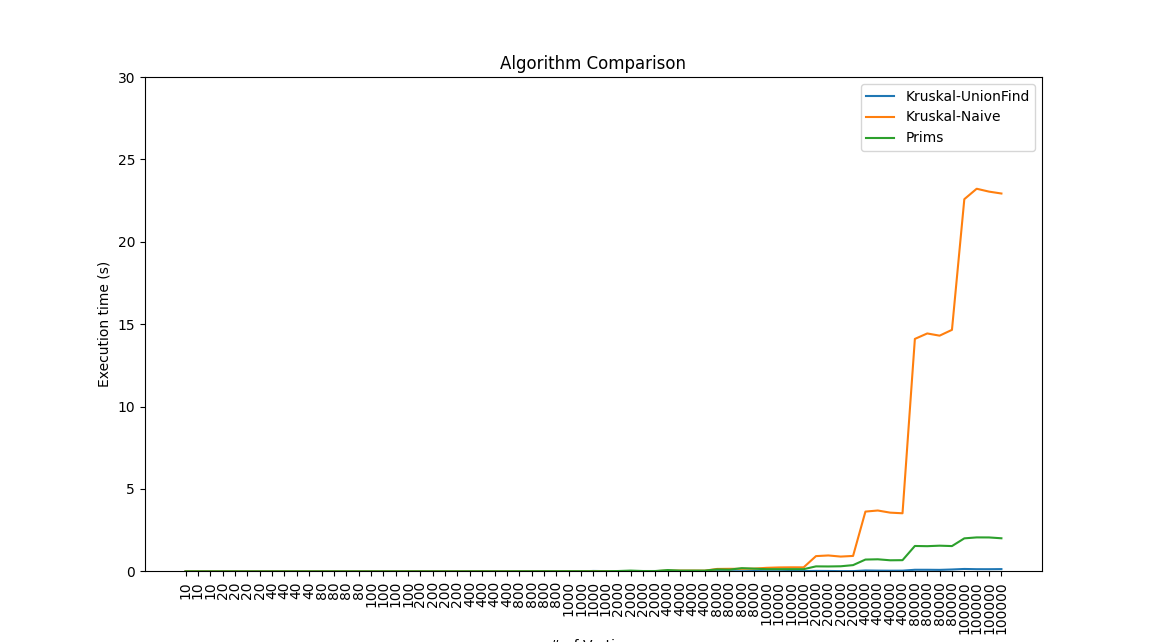
\includegraphics[width=19cm]{Img/AlgorithmComparison_Graph.png}
	\caption{Comparison between the performances of the three algorithms }
	\label{comparison}
\end{figure}

\pagebreak


\end{document}